% problems: fundamentals of probability

\section*{Problems}

The standard deck of cards is divided into four suits, two red and two black:
\begin{itemize}
	\item Spades $\spadesuit$,
	\item Hearts $\heartsuit$,
	\item Diamonds $ \diamondsuit$,
	\item Clubs $\clubsuit$
\end{itemize}

Each suit consists of 13 cards, of which 9 are number cards and 4 are face cards/aces. They are ordered from lowest to highest rank as follows: A, 2, 3, 4, 5, 6, 7, 8, 9, 10, J, Q, and K.

\begin{figure}[ht]
	\centering
	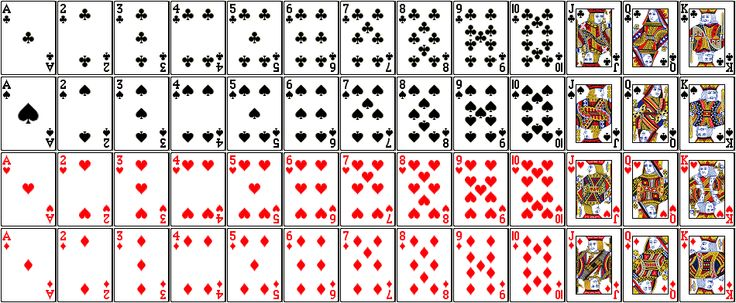
\includegraphics[width=10cm]{./pe/deck.jpg}
	\caption{Standard English deck}
	\label{fig:2.3.3}
\end{figure}


\subsection{Problem Statements}

\subsubsection*{1. Fundamental Level (Simple / Direct)}

\begin{problem}
	\sidenote{\href{https://youtu.be/4LdLWpQIcBQ}{See also the online solution.}}
	\label{prob:2.3.1}
	A card is drawn at random from a standard English deck of 52 cards. Formally describe the sample space $S$ if both suits and ranks are considered.
\end{problem}

\begin{problem}
	\sidenote{\href{https://youtu.be/S9VFhMWVyu4}{See also the online solution.}}
	\label{prob:2.3.2}
	Suppose $A$ is the event \texttt{``a king is drawn''} or simply $\set{K},$ while $B$ is the event \texttt{``a club is drawn''} or simply $\set{\clubsuit}$. Describe in words the meaning of the following combined events: 
	\begin{enumerate}
		\item $A\cup B$ 
		\item $A\cap B$ 
		\item $A \cup B'$ 
		\item $A' \cup B'$ 
		\item $A - B$ 
		\item $A'-B'$ 
		\item $(A\cap B) \cup (A\cap B')$
	\end{enumerate}
\end{problem}

\begin{problem}
	\label{prob:2.3.5}
	Find the exact probability that in two rolls of a fair 6-sided die, at least one 4 is obtained on either of the two rolls.
\end{problem}

\subsubsection*{2. Operational Level (Intermediate / Developmental)}

\begin{problem}
	\label{prob:2.3.3}
	From a well-shuffled standard English deck, 2 cards are drawn successively. Find the probability that both cards are aces if:
	\begin{enumerate}
		\item The first card is returned to the deck before the second draw (with replacement).
		\item The first card is not returned to the deck (without replacement).
	\end{enumerate}
\end{problem}

\begin{problem}
	\label{prob:2.3.4}
	In a container there are 6 red balls, 4 white balls, and 5 blue balls. Three balls are drawn successively at random. Find the probability that they are drawn specifically in the order red, white, and blue if:
	\begin{enumerate}
		\item Each ball is returned to the container after being drawn.
		\item The balls are not returned to the container.
	\end{enumerate}
\end{problem}

\begin{problem}
	\label{prob:2.3.6}
	When rolling two fair dice simultaneously, determine the probability of \emph{not} obtaining a total sum of 7 points nor 11 points.
\end{problem}

\subsubsection*{3. Analytical Level (Advanced / Connection)}

\begin{problem}
	\label{prob:2.3.7}
	Starting exclusively from Kolmogorov's three axioms ($P(A) \ge 0$, $P(S)=1$, and countable additivity for mutually exclusive events), prove the general addition rule for two arbitrary events $A, B \subset S$:
	\begin{align}
		P(A \cup B) = P(A) + P(B) - P(A \cap B).
	\end{align}
\end{problem}

\begin{problem}
	\label{prob:2.3.8}
	Let $A \subset S$ be an event and $A'$ its complement. Algebraically prove using Kolmogorov's axioms that:
	\begin{enumerate}
		\item $P(A') = 1 - P(A)$.
		\item The probability of the impossible or empty event is zero: $P(\emptyset) = 0$.
	\end{enumerate}
\end{problem}

\subsubsection*{4. Challenging Level (Expert / Deep Deduction)}

\begin{problem}
	\label{prob:2.3.9}
	\begin{enumerate}
		\item Prove by mathematical induction Boole's Inequality (subadditivity bound) for the union of $n$ arbitrary events:
		\begin{align}
			P\left( \bigcup_{i=1}^{n} A_{i} \right) \le \sum_{i=1}^{n} P(A_{i}).
		\end{align}
		\item Using the addition rule, deduce Bonferroni's Inequality for the intersection of two events:
		\begin{align}
			P(A \cap B) \ge P(A) + P(B) - 1.
		\end{align}
	\end{enumerate}
\end{problem}

\begin{problem}
	\label{prob:2.3.10}
	At a gala dinner, $n$ guests leave their hats at the cloakroom. At the end of the evening, the attendant returns the $n$ hats completely at random. Let $A_{i}$ be the event that the $i$-th guest receives their own hat ($i=1,2,\dots,n$).
	\begin{enumerate}
		\item Using the inclusion-exclusion principle for probabilities, prove the general formula for the probability that \emph{at least one} of the guests receives their correct hat:
		\begin{align}
			P\left( \bigcup_{i=1}^{n} A_{i} \right) = \sum_{k=1}^{n} \frac{(-1)^{k-1}}{k!}.
		\end{align}
		\item Calculate the limit of this probability as the number of guests grows indefinitely ($n \to \infty$) and numerically verify its asymptotic behavior.
	\end{enumerate}
\end{problem}


\subsection{Detailed Solutions}

\subsubsection*{1. Fundamental Level (Simple / Direct)}

\begin{solproblem}
	The solution is given by the Cartesian product of the set of suits:
	\begin{align}
		P = \set{\spadesuit, \heartsuit, \diamondsuit, \clubsuit},
	\end{align}
	whose cardinality is 4, and the set of ranks:
	\begin{align}
		R = \set{\text{A}, 2, 3, 4, 5, 6, 7, 8, 9, 10, \text{J}, \text{Q}, \text{K}},
	\end{align}
	whose cardinality is 13.
	The complete sample space is $S = P \times R$, containing exactly $4 \times 13 = 52$ equally likely sample points.
\end{solproblem}

\begin{solproblem}
	\begin{enumerate}
		\item $A \cup B$: Either a king or a club is drawn (or both).
		\item $A \cap B$: A king and a club are drawn simultaneously (specifically, the King of Clubs).
		\item $A \cup B'$: Either a king is drawn or a card that is not a club is drawn (equivalent to: if it is a club, it must be a king).
		\item $A' \cup B'$: Either not a king or not a club is drawn (by De Morgan's Law, this is the complement of drawing the King of Clubs).
		\item $A - B$: A king that is not a club is drawn ($A \cap B'$).
		\item $A' - B'$: A card that is not a king and is a club is drawn ($A' \cap B$).
		\item $(A \cap B) \cup (A \cap B')$: Either a king of clubs or a king of another suit is drawn. By distributivity of intersection over union, this simply equals event $A$ (\texttt{``a king is drawn''}).
	\end{enumerate}
\end{solproblem}

\begin{solproblem}
	The sample space for rolling two dice consists of $6 \times 6 = 36$ equally likely ordered pairs.
	We calculate using the complementary event: the event $E'$ of \emph{not} obtaining any 4 on either die means that each die can land on any of the 5 remaining faces ($\{1,2,3,5,6\}$).
	
	The number of favorable cases for the complement $E'$ is $5 \times 5 = 25$.
	Therefore, the probability of event $E$ (\texttt{``at least one 4''}) is:
	\begin{align}
		P(E) = 1 - P(E') = 1 - \dfrac{25}{36} = \dfrac{11}{36} \approx 0.3056.
	\end{align}
\end{solproblem}

\subsubsection*{2. Operational Level (Intermediate / Developmental)}

\begin{solproblem}
	In a 52-card deck there are 4 aces ($A$).
	\begin{enumerate}
		\item \textbf{With replacement:} The deck composition is identical for both draws:
		\begin{align}
			P(A_1 \cap A_2) = P(A_1) \cdot P(A_2) = \dfrac{4}{52} \times \dfrac{4}{52} = \dfrac{1}{13} \times \dfrac{1}{13} = \dfrac{1}{169} \approx 0.0059.
		\end{align}
		
		\item \textbf{Without replacement:} The second draw depends on having drawn an ace on the first draw (3 aces remain among 51 cards):
		\begin{align}
			P(A_1 \cap A_2) = P(A_1) \cdot P(A_2 | A_1) = \dfrac{4}{52} \times \dfrac{3}{51} = \dfrac{1}{13} \times \dfrac{1}{17} = \dfrac{1}{221} \approx 0.0045.
		\end{align}
	\end{enumerate}
\end{solproblem}

\begin{solproblem}
	The container holds $6 + 4 + 5 = 15$ balls in total.
	\begin{enumerate}
		\item \textbf{With replacement:} The three color events are independent:
		\begin{align}
			P(R_1 \cap B_2 \cap A_3) = \dfrac{6}{15} \times \dfrac{4}{15} \times \dfrac{5}{15} = \dfrac{2}{5} \times \dfrac{4}{15} \times \dfrac{1}{3} = \dfrac{8}{225} \approx 0.0356.
		\end{align}
		
		\item \textbf{Without replacement:} The container's total decreases by 1 at each step:
		\begin{align}
			P(R_1 \cap B_2 \cap A_3) &= P(R_1) \cdot P(B_2 | R_1) \cdot P(A_3 | R_1 \cap B_2) \\
			&= \dfrac{6}{15} \times \dfrac{4}{14} \times \dfrac{5}{13} = \dfrac{2}{5} \times \dfrac{2}{7} \times \dfrac{5}{13} = \dfrac{4}{91} \approx 0.0440.
		\end{align}
	\end{enumerate}
\end{solproblem}

\begin{solproblem}
	The sample space for rolling two dice has $36$ equally likely simple events.
	We identify pairs whose sum is 7 or 11:
	\begin{itemize}
		\item Sum equals 7: $\set{(1,6), (2,5), (3,4), (4,3), (5,2), (6,1)}$ (6 events).
		\item Sum equals 11: $\set{(5,6), (6,5)}$ (2 events).
	\end{itemize}
	Since the events \texttt{``sum of 7''} and \texttt{``sum of 11''} are mutually exclusive, the total number of cases where either occurs is $6 + 2 = 8$.
	
	Therefore, the probability of the complementary event (obtaining neither 7 nor 11) is:
	\begin{align}
		P(\text{neither 7 nor 11}) = 1 - \dfrac{8}{36} = \dfrac{28}{36} = \dfrac{7}{9} \approx 0.7778.
	\end{align}
\end{solproblem}

\subsubsection*{3. Analytical Level (Advanced / Connection)}

\begin{solproblem}
	From partition theory, we can express the union set $A \cup B$ and set $A$ as unions of mutually exclusive (disjoint) sets:
	\begin{align}
		A \cup B &= A \cup (B \backslash A) \\
		B &= (A \cap B) \cup (B \backslash A)
	\end{align}
	By Kolmogorov's third axiom (countable additivity for disjoint sets):
	\begin{align}
		P(A \cup B) &= P(A) + P(B \backslash A) \label{eq:prob_u1} \\
		P(B) &= P(A \cap B) + P(B \backslash A) \implies P(B \backslash A) = P(B) - P(A \cap B) \label{eq:prob_u2}
	\end{align}
	Substituting equation (\ref{eq:prob_u2}) into equation (\ref{eq:prob_u1}):
	\begin{align}
		P(A \cup B) = P(A) + P(B) - P(A \cap B).
	\end{align}
	This identity proves the general addition rule in probability without relying on finite counting.
\end{solproblem}

\begin{solproblem}
	\begin{enumerate}
		\item By definition of complement, $A \cup A' = S$ and $A \cap A' = \emptyset$. Since they are disjoint events, applying Kolmogorov's third axiom and second axiom ($P(S)=1$):
		\begin{align}
			P(S) &= P(A \cup A') = P(A) + P(A') \\
			1 &= P(A) + P(A') \implies P(A') = 1 - P(A).
		\end{align}
		
		\item For the empty set, observe that $S \cup \emptyset = S$ and $S \cap \emptyset = \emptyset$ (they are disjoint). By axiomatic additivity:
		\begin{align}
			P(S) = P(S \cup \emptyset) = P(S) + P(\emptyset).
		\end{align}
		Subtracting $P(S)$ from both sides (since $P(S)=1$ is a finite number), we obtain:
		\begin{align}
			P(\emptyset) = 0.
		\end{align}
	\end{enumerate}
\end{solproblem}

\subsubsection*{4. Challenging Level (Expert / Deep Deduction)}

\begin{solproblem}
	\begin{enumerate}
		\item \textbf{Boole's Inequality by induction:}
		For $n=1$, the statement holds trivially ($P(A_1) \le P(A_1)$).
		For $n=2$, we know from the general addition rule that $P(A_1 \cup A_2) = P(A_1) + P(A_2) - P(A_1 \cap A_2)$. By the first axiom, $P(A_1 \cap A_2) \ge 0$, thus:
		\begin{align}
			P(A_1 \cup A_2) \le P(A_1) + P(A_2).
		\end{align}
		Suppose the inequality holds true for $k$ events (inductive hypothesis). For $k+1$ events, grouping the last event:
		\begin{align}
			P\left( \bigcup_{i=1}^{k+1} A_i \right) = P\left( \left[\bigcup_{i=1}^{k} A_i\right] \cup A_{k+1} \right) \le P\left( \bigcup_{i=1}^{k} A_i \right) + P(A_{k+1}) \le \sum_{i=1}^{k} P(A_i) + P(A_{k+1}) = \sum_{i=1}^{k+1} P(A_i).
		\end{align}
		This proves the inequality by induction for all $n \ge 1$.
		
		\item \textbf{Bonferroni's Inequality:}
		Starting from $P(A \cup B) = P(A) + P(B) - P(A \cap B)$, and knowing from the axioms that any probability satisfies $P(A \cup B) \le 1$:
		\begin{align}
			P(A) + P(B) - P(A \cap B) &\le 1 \\
			P(A \cap B) &\ge P(A) + P(B) - 1.
		\end{align}
	\end{enumerate}
\end{solproblem}

\begin{solproblem}
	\begin{enumerate}
		\item \textbf{Inclusion-exclusion principle applied to coincidences:}
		The probability that a person receives their correct hat corresponds to the fraction of permutations fixing at least one element.
		For a single index $i$, $P(A_i) = \frac{(n-1)!}{n!} = \frac{1}{n}$.
		For two individuals $i < j$, $P(A_i \cap A_j) = \frac{(n-2)!}{n!} = \frac{1}{n(n-1)}$.
		In general, for the intersection of $k$ individuals simultaneously, the probability is $\frac{(n-k)!}{n!}$.
		
		The general inclusion-exclusion principle for $n$ events states:
		\begin{align}
			P\left( \bigcup_{i=1}^{n} A_i \right) = \sum_{i=1}^n P(A_i) - \sum_{i<j} P(A_i \cap A_j) + \sum_{i<j<l} P(A_i \cap A_j \cap A_l) - \dots + (-1)^{n-1} P(A_1 \cap \dots \cap A_n).
		\end{align}
		The number of ways to choose $k$ people out of $n$ is $\binom{n}{k}$. Multiplying the joint probability by the number of combinations in the $k$-th term yields:
		\begin{align}
			S_k = \binom{n}{k} \cdot \frac{(n-k)!}{n!} = \frac{n!}{k!(n-k)!} \cdot \frac{(n-k)!}{n!} = \frac{1}{k!}.
		\end{align}
		Substituting each partial sum $S_k$ into the main formula:
		\begin{align}
			P\left( \bigcup_{i=1}^{n} A_i \right) = \sum_{k=1}^{n} (-1)^{k-1} S_k = \sum_{k=1}^{n} \frac{(-1)^{k-1}}{k!} = 1 - \frac{1}{2!} + \frac{1}{3!} - \dots + \frac{(-1)^{n-1}}{n!}.
		\end{align}
		
		\item \textbf{Asymptotic limit:}
		Recall the Taylor series expansion for the exponential function evaluated at $x = -1$:
		\begin{align}
			e^{-1} = \sum_{k=0}^{\infty} \frac{(-1)^k}{k!} = 1 - 1 + \frac{1}{2!} - \frac{1}{3!} + \frac{1}{4!} - \dots = 1 - \sum_{k=1}^{\infty} \frac{(-1)^{k-1}}{k!}.
		\end{align}
		Therefore, as the number of guests grows ($n \to \infty$):
		\begin{align}
			\lim_{n \to \infty} P\left( \bigcup_{i=1}^{n} A_i \right) = 1 - e^{-1} = 1 - \frac{1}{e} \approx 0.63212.
		\end{align}
		Remarkably, for any dinner with $n \ge 6$ guests, the probability that at least one person receives their own hat stabilizes almost exactly at 63.21\%.
	\end{enumerate}
\end{solproblem}
